\section{Instructions for GUI} \label{app_sec:instructions}
\subsection{Running the software}
\begin{enumerate}
   \item Open the shortcut CAD.m with MATLAB. Ensure your workspace root folder contains CAD.m and the functions folder
   \item Run CAD.m from MATLAB. This should open the O-Crab user interface
   \item Select your desired configuration either by sliding the sliders, or by entering a value in the text boxes. The values are restricted by the minimum and maximum determined for each option. See Figure \ref{fig:userInterface} for more information.
   \item Click the "Compute!" button. Note: If no value is entered, the minimum for all options will be selected.
   \item Wait for the  "Calculations Complete, Solid Work can now be updated" message to appear in the MatLab command prompt before rebuilding the SolidWorks Assembly.
        \begin{itemize}
            \item Note: The information above in the MatLab command prompt are properties of the robot which cannot be shown in the SolidWorks assembly.
        \end{itemize}
        \begin{itemize}
            \item Note: Do not change the input parameters while the program is running
        \end{itemize}
        \item Open the shortcut to the O-Crab.SLDASM file from the root folder to open the assembly in SolidWorks.
   \item Rebuild the SolidWorks assembly. 
       \begin{itemize}
            \item Note: It is normal for errors to occur on the first rebuild. Without running the MatLab code again, rebuild the SolidWorks assembly a second time if needed. Occasionally, one of the bellow runs through a rebuild issue related to its geometry although every bellow uses the same geometry. That specific bellow can be suppressed if it prevents the rest of the assembly from rebuilding properly.
        \end{itemize}
    \item The SolidWorks assembly is now ready. The one leg without the bellow is movable and restricted between the normal walking angle ranges.
    \item To continue testing different combinations, change the input parameters and select "Compute!" again. 
    \begin{itemize}
            \item Note: Do not modify the CAD model while the program is running
        \end{itemize}
\end{enumerate}

\subsection{Debugging}
\begin{itemize}
            \item If either the CAD.m or O-Crab.SLDASM shortcuts do not work, you can open them directly from \texttt{WR2A/MATLAB/CAD.m} or \texttt{WR2A/SolidWorks/Parts/Parametrized/O-Crab.SLDASM}.
            \item If any errors are thrown while running CAD.m, the functions folder (and sub-folders) are likely not added to the path. Ensure your MATLAB root folder is WR2A/MATLAB and add all folders and subfolders.
            \item If the SolidWorks assembly does not build properly after parameterizing, rebuild.
\end{itemize}

\begin{figure}[H]
    \centering
    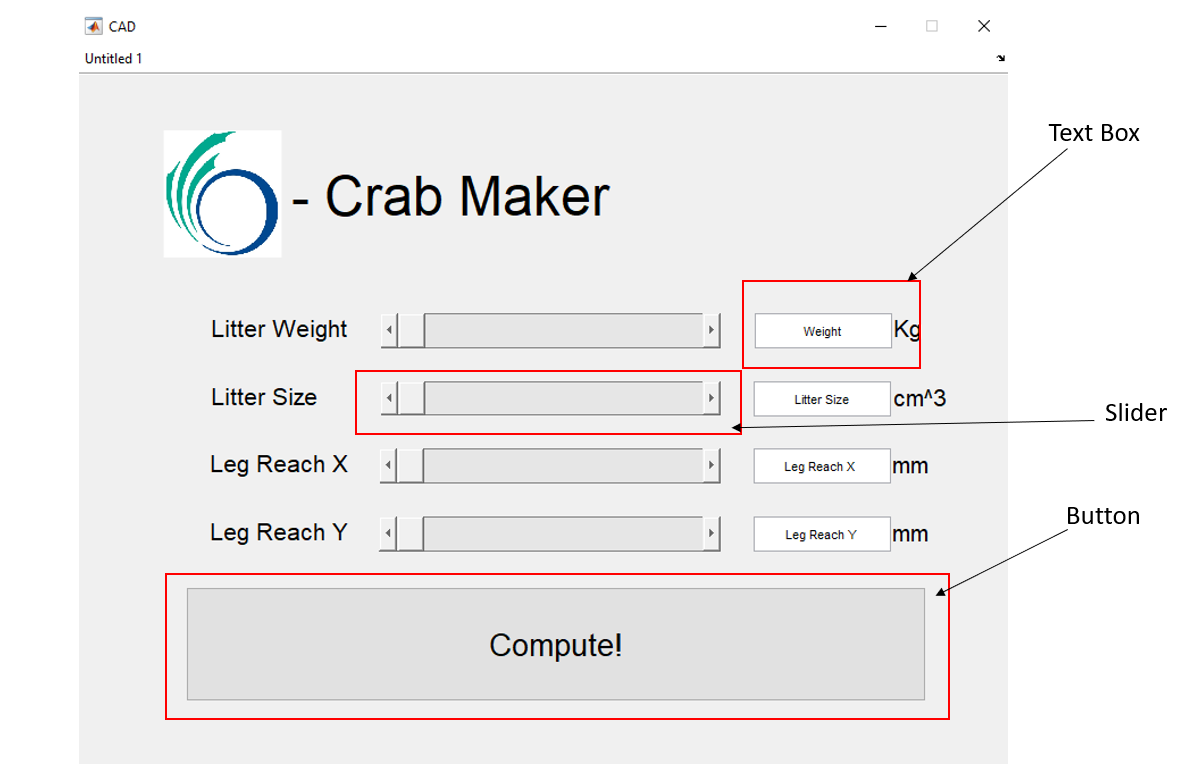
\includegraphics[width=1\textwidth]{6_Appendices/Instruction/GUI_Instructions.PNG}
    \caption{User Interface}
    \label{fig:userInterface}
\end{figure}{}
